\begin{example}
    Consider the following network where we want to check a blacklist
    property, i.e. no packets arrive at $d$:
    \begin{center}
        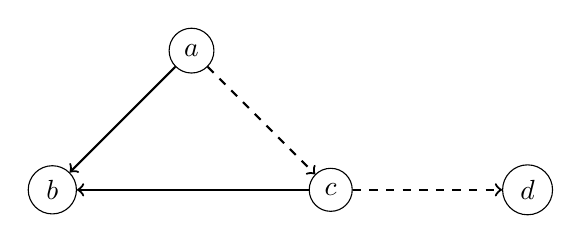
\begin{tikzpicture}[node distance={25mm},
                main/.style = {draw, circle},
                s/.style = {->,thick},
                d/.style = {->,thick,dashed} ]
            \node[main] (b) {$b$};
            \node[main] (a) [above right of=b] {$a$};
            \node[main] (c) [below right of=a] {$c$};
            \node[main] (d) [right of=c] {$d$};
            \draw[s] (a) -- (b);
            \draw[d] (a) -- (c);
            \draw[s] (c) -- (b);
            \draw[d] (c) -- (d);
        \end{tikzpicture}
    \end{center}
    We define this network using the following DyNetKAT term:
    \begin{align*}
        S_{xy}  & = l = x \cdot l \la y              \\
        P       & = u!S_{ac}                         \\
        Q       & = u!S_{cd}                         \\
        N_{x,y} & = (S_x+S_y)^* \oplus u?x';N_{x',y}
        \oplus u?y';N_{x,y'}                         \\
        SDN     & = N_{ab,cb} \parallel P \parallel Q
    \end{align*}
    We may rewrite the terms as follows:
    \begin{align*}
        N_{ab,cb} & = (S_{ab} + S_{cb})^* \oplus u?S_{ac};N_{ac,cb}
        \oplus u?S_{cd};N_{ab,cd}                                   \\
        N_{ac,cb} & = (S_{ac}+S_{cb})^* \oplus u?S_{cd};N_{ac,cd}   \\
        N_{ab,cd} & = (S_{ab}+S_{cd})^* \oplus u?S_{ac};N_{ac,cd}   \\
        N_{ac,cd} & = (S_{ac}+S_{cd})^*
    \end{align*}
    Given a packet $\sigma$ where $\sigma(l) = a$ we can replace NetKAT
    policies with actions of the form $(\sigma, \sigma')$.
    In this network we denote the action $(\sigma, \sigma')$
    with $xy$ where $\sigma(l) = x$ and $\sigma'(l) = y$.
    Let $N'_{x,y}$ be the term where we replaced NetKAT policies with
    actions of the form $(\sigma,\sigma')$ and let we use $p,p',q,q'$ to
    denote the actions $u?S_{ac},u!S_{ac},u?S_{cd},u!S_{cd}$.
    Thus we have:
    \begin{align*}
        SDN' & = N'_{ab,cb} \parallel P \parallel Q \\
        P' & = p' \\
        Q' & = q' \\
        N'_{ab,cb} & = ab \oplus p;N'_{ac,cb} \oplus q;N'_{ab,cd} \\
        N'_{ac,cb} & = ac \oplus ab \oplus q;N'_{ac,cd}   \\
        N'_{ab,cd} & = ab \oplus p;N'_{ac,cd}             \\
        N'_{ac,cd} & = ac \oplus ad 
    \end{align*}
    \begin{center}
        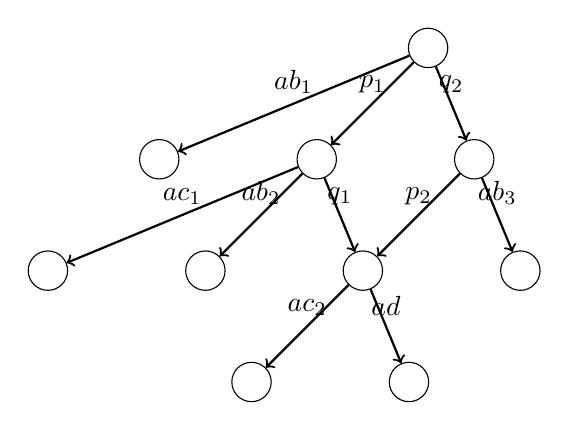
\begin{tikzpicture}[node distance={20mm},
                main/.style = {draw, circle,minimum width=5mm},
                s/.style = {->,thick}]
            \node[main] (s1) {};
            \node[main] (s3) [below left of=s1] {};
            \node[main] (s2) [left of=s3] {};
            \node[main] (s4) [right of=s3] {};
            \node[main] (s5) [below left of=s2] {};
            \node[main] (s6) [right of=s5] {};
            \node[main] (s7) [right of=s6] {};
            \node[main] (s8) [right of=s7] {};
            \node[main] (s9) [below left of=s7] {};
            \node[main] (s10) [right of=s9] {};
            \draw[s] (s1) -- node[above]{$ab_1$} (s2);
            \draw[s] (s1) -- node[above]{$p_1$}(s3);
            \draw[s] (s1) -- node[above]{$q_2$}(s4);
            \draw[s] (s3) -- node[above]{$ac_1$}(s5);
            \draw[s] (s3) -- node[above]{$ab_2$}(s6);
            \draw[s] (s3) -- node[above]{$q_1$}(s7);
            \draw[s] (s4) -- node[above]{$p_2$}(s7);
            \draw[s] (s4) -- node[above]{$ab_3$}(s8);
            \draw[s] (s7) -- node[above]{$ac_2$}(s9);
            \draw[s] (s7) -- node[above]{$ad$}(s10);
        \end{tikzpicture}
    \end{center}
    We may define the event structure $\mathrm{E} = (E,\#,\vdash)$ for $SDN'$ 
    where we have:
    \begin{align*}
        E = \s{ab_1,ab_2,ab_3,ac_1,ac_2,ad,p_1,p_2,q_1,q_2} \\
    \end{align*}
    Enabling relation the least one that satisfies:
    \begin{align*}
        & \e \vdash ab_1, \e \vdash p_1, \e \vdash q_2,
        \s{p_1} \vdash ac_1, \s{p_1} \vdash ab_2, \s{p_1} \vdash q_1,
        \s{q_1} \vdash p_2, \s{q_1} \vdash ab_3 \\
        & \s{p_1,q_1} \vdash ac_2, \s{p_1,q_1} \vdash ad,
        \s{p_2,q_2} \vdash ac_2, \s{p_2,q_2} \vdash ad
    \end{align*}
    And conflict relation the least one where:
    \begin{align*}
        \forall i,j,k. j \neq k \Rightarrow e_{i,k} \# e_{j,k} \\
    \end{align*}
    Given an event structure $\mathrm{E} = (E,\#,\vdash)$, we define a safety
    property $\mathcal{P}$ as a subset of $\mathcal{F}(\mathrm{E})$.
    The safety property here is $d$ is being blacklist. 
    Thus, we define $ p \subseteq \mathcal{F}(\mathrm{E})$ to be the set of 
    configurations that do not contain an event of forwarding a packet to $d$.
    More formally we define $p$ as follows:
    \begin{align*}
        p = \s{s \subseteq E| \forall e \in s.  l(e) = (\sigma, \sigma')
         \Rightarrow \sigma'(l) \neq d }
    \end{align*}
    Finally, we can consider the set $\mathcal{P}(E) \setminus p$ as the 
    set of configurations for which we want to find the cause.
    Here, let $s = \mathcal{P}(E) \setminus p$.
    For our blacklist property $s$ contains all subsets of $E$ that contain $ad$.
    We wish to define nonexistence of a conflict between $p_1$ and $q_1$ 
    as a cause.
    We consider the witness $(C(p_2,q_2),\T,\T)$.
    If we set both $C(p_1,q_1)$ and $C(p_2,q_2)$ to true, then $ES$ for any 
    configuration $\sigma$ of $ES$ we have $\s{p_1,q_1} \not \in \sigma$ and
    $\s{p_1,q_2} \not \in \sigma$. Now, since $ad$ is only enabled either by
    $\s{p_1,q_1}$ or $\s{p_2,q_2}$, we can conclude that $ES$ can not have a
    configuration containing $ad$.
    For AC2(b), if we only set $C(p_2,q_2)$ to true, still ${p_1,q_1,ad}$ is 
    a configuration of $ES$ under any reset of other variables to their actual 
    values.
    Thus AC conditions are satisfied and we can declare $C(p_1,q_1)$ as a cause of
    the violation of the blacklist property.

\end{example}